\chapter{System design}

\todo{divide and conquer?}

Designing a system requires deep understanding of the \todo{problem space/use cases/task definition} to then create a solution.
The better the knowledge of existing system is, the more easier it is to take advantage of established solutions and evade known pitfalls.
This chapter will concentrate on the big \todo{headaches} by analyzing and comparing them to existing or similar solutions and develop a solution with the help of the gathered knowledge.

\section{Execution Management}

\subsection{Remote Execution}

In this approach, the job is executed on a remote machine and not on the same node which has the responsibility in managing the execution.
Continuous Integration (CI) platform Jenkins\cite{jenkins:main} as well as GitLab\cite{gitlab:main} do offer this approach.
The so called slave node (Jenkins) or runner (GitLab) is accessed by the CI through a common interface (SSH in these cases) to start the job execution.
Jenkins and GitLab even copy a custom binary onto the slave node, that is then managing the execution on the remote machine locally.
This is due to the complexity in executing the job for a given configuration as well as being able to continue the execution on disconnects or maintenance reboots of the master machine.

In this scenario, the CI instance requires and stores login credentials for every remote machine to be able to login whenever needed.
The system administrator therefore has to create a new user account on the remote machine, install required programs and environments (bot Jenkins and GitLab require an JRE\footnote{Java Runtime Environment}).
In case of an security breach on the CI instance, the attacker is also able to login on all remote nodes and execute arbitrary programs as well \todo{there is probably a great article about an issue like this!?}.

\todo{WRONG, on GitLab YOU need to intall/setup the runner}

GitLab follows another approach, the system administrator has to manually install the GitLab Runner\footnote{\todo{cite}} on a slave node and is then able to add this runner to a Project.
The security risk is somewhat similar to Jenkins: once an attacker has access to the CI instance, arbitrary code can be uploaded and executed on the remote machines. \todo{but no ssh login .... until first binary uploaded}

\todo{winslow is more secure because of docker and therefore limited access to the system, no network..?}

\subsection{Local Execution}

Executing a job locally means running the job on the same machine as the program that is watching and managing the execution.
This has the advantage of having all libraries, tools and resources already present.
But in the case of Jenkins and GitLab, this is means, each CI instance is separate from the others.
There is no integration between those instance in this configuration.
What is missing Jenkins and GitLab here is the capability to decentralize their core task of managing projects, resources and executions.


\subsection{Decision for Winslow}

\section{Communication and Synchronization}

For the instances of Winslow, communication and especially synchronization is very important.
Without proper coordination, race conditions could cause stages to be started multiple times simultaneously, corrupt workspaces, configuration or project files.
While starting too many stage executions are only wasting resources, data corruptions can lead to unrecoverable damage.

Before synchronization can be achieved, communication must be possible.
There are multiple ways to exchange data for systems that do not share the same process or machine.
The most flexible implementation can be achieved by implementing a custom protocol on a raw TCP socket which allows to exchange blobs\footnote{\todo{Binary Large Objects}} between exactly two nodes.
For a blob or message to reach all nodes, there needs to be connections to all other nodes \todo{great mafs N*N, N*(N-1) or whatever}, a centralized broker (introducing single point of failure), or another connection organization such as a tree structure.
Having many connections can stress the hosting system while complex structures require additional development and maintenance overhead in non-problem related domains.
To not have to worry about the structure, broadcasting or multicasting blobs to all nodes could be an alternative.
But UDP messages are not guaranteed to be delivered and introduce further overhead to detect the need to retransmit a blob.
Because of these concerns, the idea of a custom implementation on top of a raw TCP Socket was abandoned, instead alternatives were investigated.


https://docs.microsoft.com/de-de/azure/architecture/microservices/design/interservice-communication


raw TCP (how to connect, centralized? star? tree?) centralized works towards -> centralized master node
broadcast?
microservice REST
event bus? kafka
messaging queue mqtt
NFS provides filesystem, filesystems are kind of standardized

https://kafka.apache.org/protocol

Apache Kafka \todo{CITE} comes very close in fulfilling all needs for a communication system.
It is open source, distributed and is focused on data and event streams.
But it introduces a dependency on the project.
It also provides functionality that is not needed, like a transaction log and persistence and replayability of all transmitted data\todo{rly?}.
Furthermore, because it is an independent service, it also requires its own TCP connection.
It is required, that this connection can be established between seemingly random nodes.
This adds another constraint to the system: the firewalls in-between the nodes must allow these connections.

Because the communication between the Winslow nodes are primarily for synchronization and not for exchange of large binary data, the previous mentioned scenarios are over fulfilling the need.
The most anticipated communication and synchronization mechanic should use and already established communication channel.
The only defined requirement yet is a common filesystem, can this be utilized to coordinate stage execution and prevent data corruption by providing basic synchronization between the compute nodes? It can!

ACID, which stands for Atomicity, Consistency, Isolation and Durability, describes the needs a database must fulfill so that it does not suffer from side effects or data corruption when executing queries.
A series of changes might not be allowed to be intercepted (atomicity), must see and result in consistent data, is not allowed to interfere with simultaneously executed queries and guarantees that once completed successfully, is in fact persistent and will not be lost (durability).

filesystem is close

DB principles: ACID

\begin{figure}[h]
	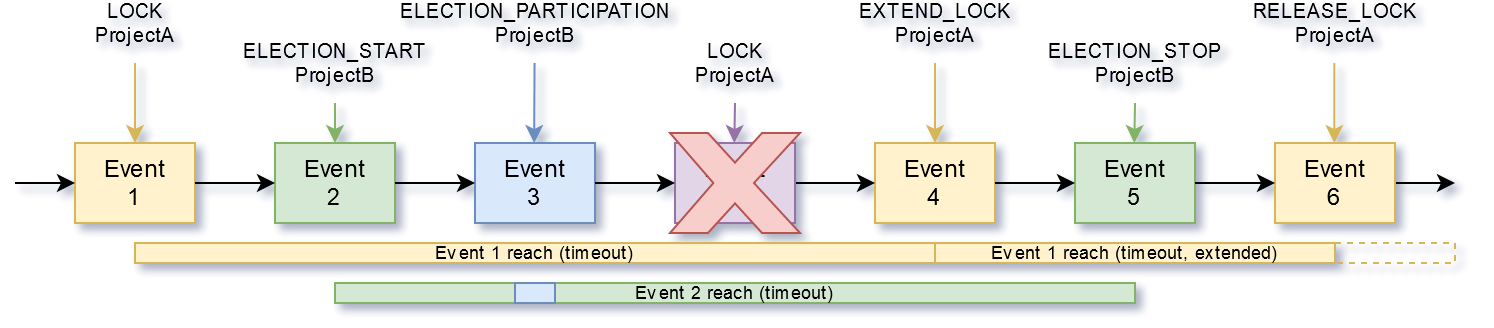
\includegraphics[width=0.9\textwidth]{events.png}
	\label{winslow:com:events}
	\caption{Sample event and lock series with lifetimes}
\end{figure}

requires common a way to exchange messages

all messages - called events - are published to all nodes

using file system as bus

clear and globally same order of events

events consist of an id, command, time, duration, subject and issuer

events might have a duration

unspoken requirement: all nodes share the same clock - or one with very little drift



\section{Storage}

\subsection{Stage storage}


Thinking about the storage organisation for the pipeline and its stages, a few expectations and concerns arise.
First of all, to redo a stage, one needs to be able to access the files that were the result of one, two or multiple stages before the current.
Sometimes a stage wants to access intermediate data produces by multiple previous stages.
Next, the input video footage needs to be accessed by multiple stages throughout the pipeline execution.
Finally, some stage results are not intermediate but final results.
\todo{examples}

The first and second concern can be solved by providing a workspace directory for each stage, that is copied from the logically previous stage.
Once the computation of a stage is completed, the workspace is considered immutable and only used to source new workspaces from.
This works fine for small intermediate results, but it does not work very well for large files - like the video footage.
Starting a new stage will take as long as the copy of multiple gigabytes on a spinning devices take (\todo{sample GB and time}), require unnecessary storage due to multiple copies and provides no benefits in an archival and version control sense, because the video footage is not altered.
So there needs to be another storage pool for input data, that is globally accessible and never changed: the global input storage pool.
Providing one further storage pool for final results (global output pool), concern number three and four are also solved.

Because the very first stage has no workspace to source its files from, on creation of the pipeline a workspace directory for the \enquote{zeroths} stage is created.
The user can then provide the very first stage with a predefined and non-empty workspace if necessary.

Because in the implementation of this project NFS was used, this also solves one further problem that was experienced in the prototyping phase: copying files on NFS (and many other network filesystems like Samba) is a client operation.
This means, the client reads the input file and writes to the output file.
Because the common network used (gigabit in this case) is slower than spinning disk sequential read/writes (network: 112 Megabytes/s in theory, divided by two because read+write on the same connection: 56 Megabytes/s, spinning enterprise disk: about 170 Megabytes/s \todo{test on johnny5}), this operation does not only take unnecessary long but also renders the network connection close to unusable for any other participant in the network that needs to use parts of the same physical route.

To ensure that the global input and the previous intermediate results are not altered, the Docker daemon is instructed to mounted them as read-only filesystems.
This makes it impossible\footnote{When there is no bug in the implementation of mount or Docker} for the stage to accidently delete or alter the wrong files\footnote{Like in this scenario, where an unexpected space in a script caued people to loose their home directory: \todo{steam rm -rf incident}}.


\begin{figure}[H]
	\centering
	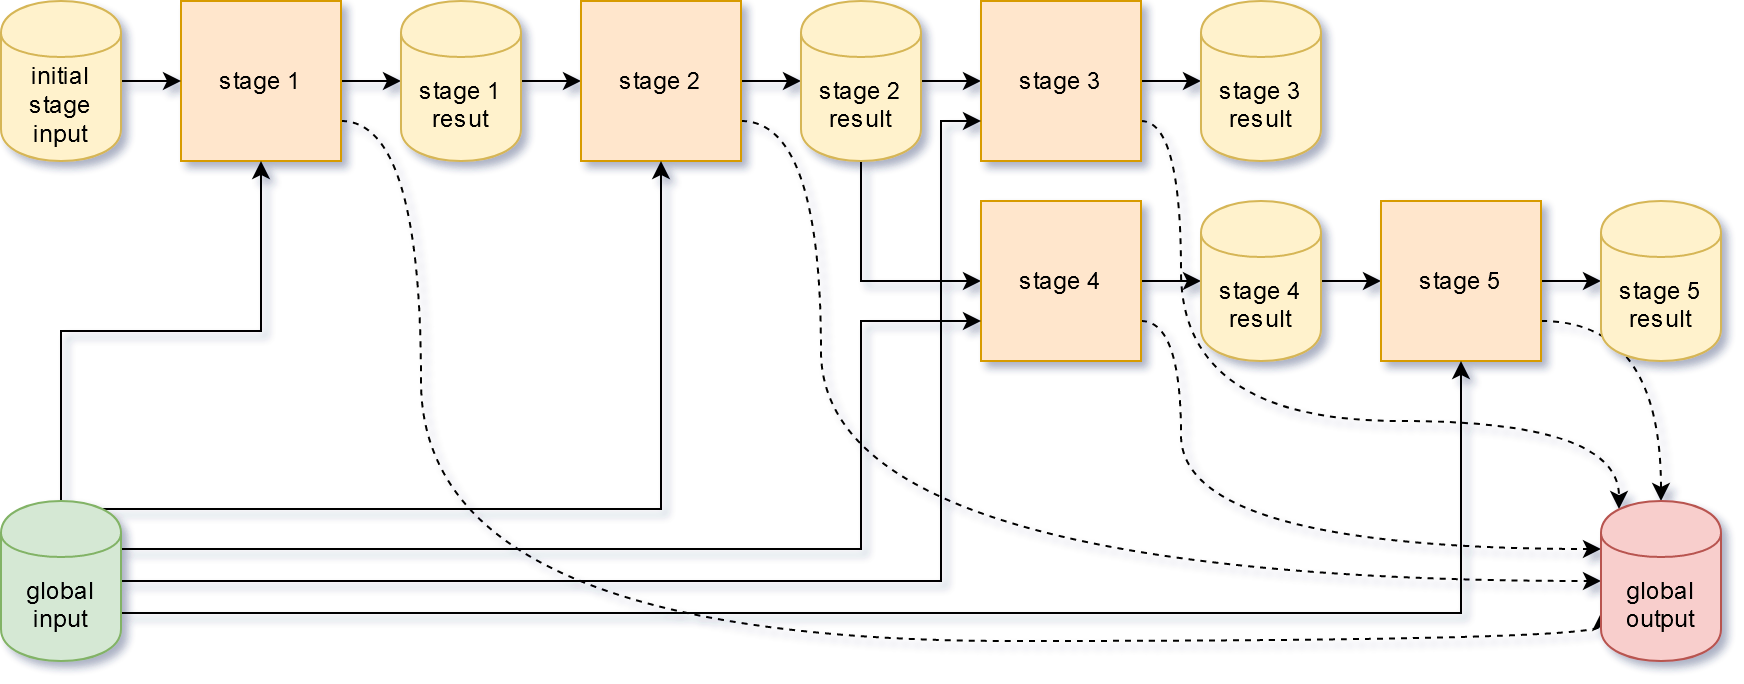
\includegraphics[width=0.9\textwidth]{stage-storage.png}
\end{figure}

In summary, the storage pool solution looks like this:

\todo{check paths}
\begin{itemize}
	\item \monospaceinline{/input} is mounted read-only from \monospaceinline{nfs-server:/winslow/workspaces/<pipeline-id>/input}
	\item \monospaceinline{/output} is mounted with write permissions from \monospaceinline{nfs-server:/winslow/workspaces/<pipeline-id>/output}
	\item \monospaceinline{/workspace} is mounted with write permissions from \monospaceinline{nfs-server:/winslow/workspaces/<pipeline-id>/<stage-id>} and was created by the copying the workspace directory of the logically previous stage
\end{itemize}

\todo{define logically previous stage -> previous stage on linear execution and ... when jumping around}



initial input

stage execution does not need to depend on the result of the exact previous



\section{Decentralized Execution - how?}

\todo{refer to kyberd presentations?}

\subsection{Every node has a connection to every other node}

\subsection{Centralized broker}

\subsection{Tree hierarchy}

\subsection{outcome}




\section{Communication and Node Management}

The system that shall be developed, is supposed to spread jobs onto execution nodes as available.
There are two main approaches in nod management and job assignment.



\subsection{Centralized Management, Remote Execution}

In the central management approach, there is always exactly one leader at any given moment in time.
It is the responsibility of this leader to decide what to execute and where to execute it.

\subsection{Decentralized Management, Local Execution}

\subsection{Combinations worth noting}

stupid:
 - centralized management, local execution
 - decentralized management, remote execution
 
combination, decentralized + some remote slaves

\section{Architecture}


\begin{figure}[H]
	\centering
	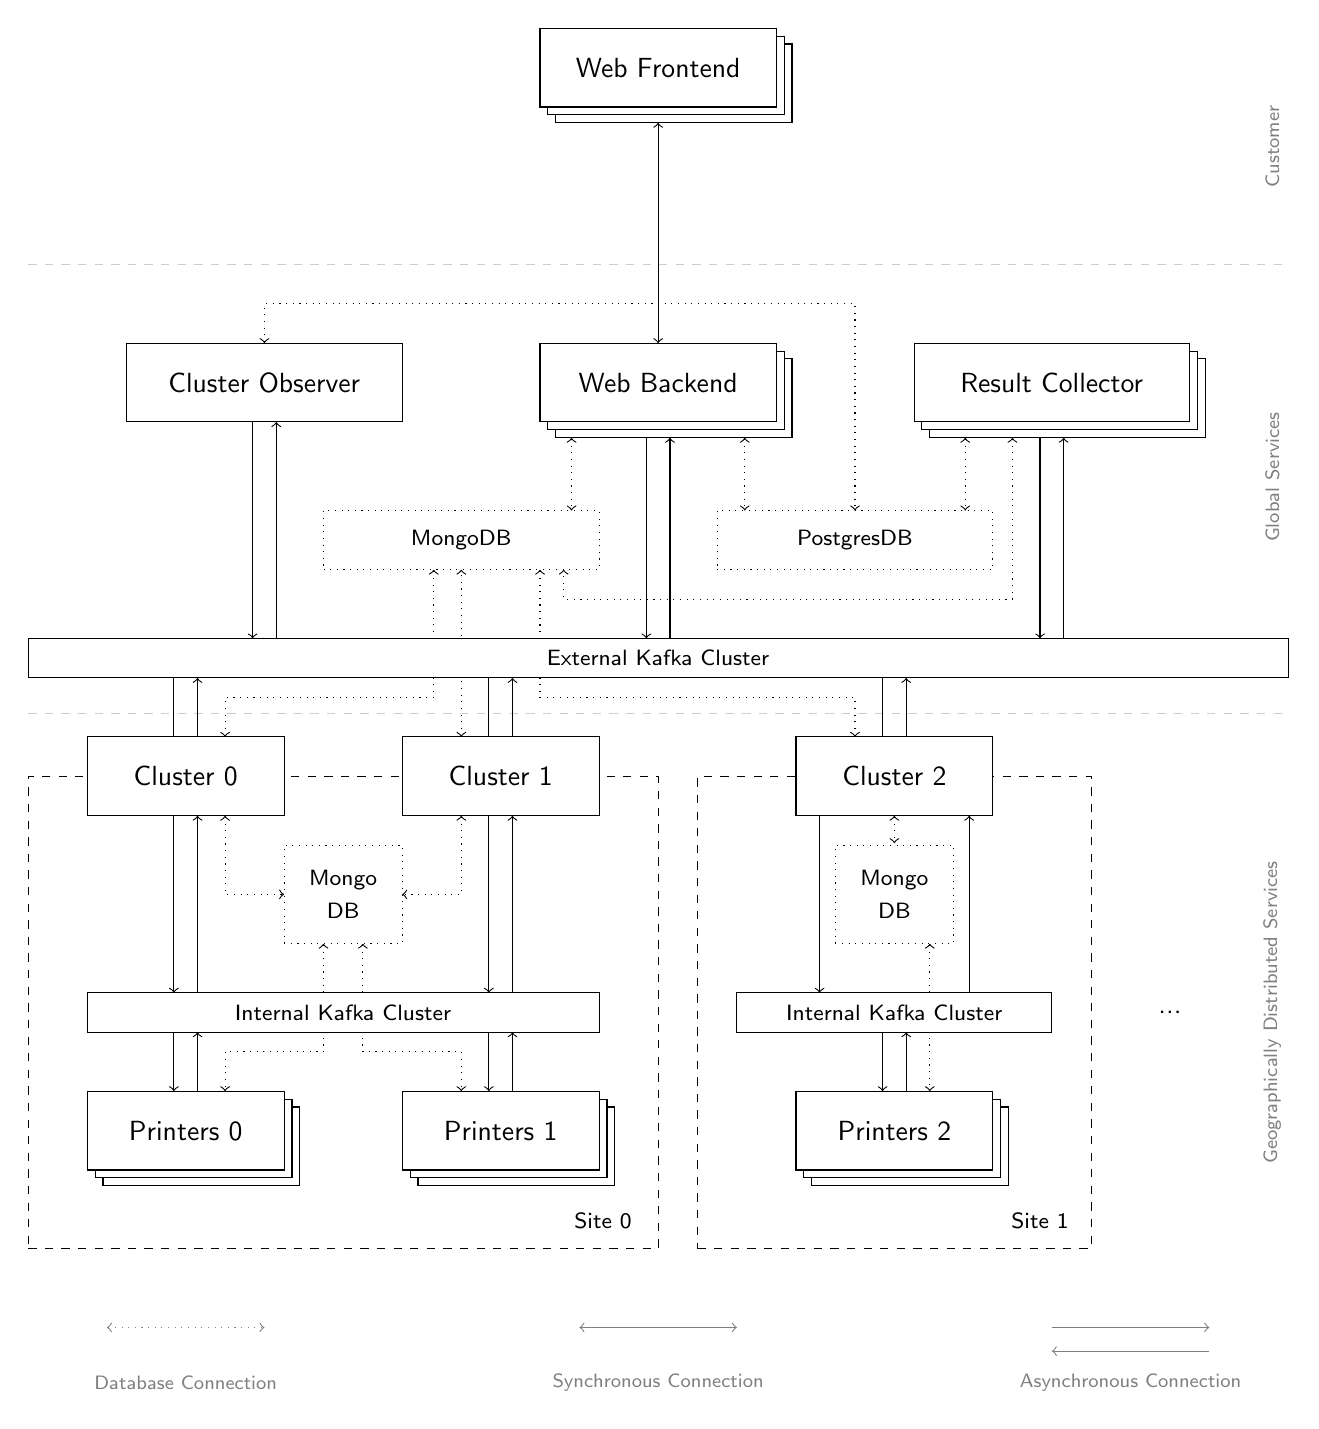
\begin{tikzpicture}
	
	\draw[-,dashed,draw=black!20!white] (-8cm, 1.5cm) to (8cm, 1.5cm);
	\draw[-,dashed,draw=black!20!white] (-8cm, -4.2cm) to (8cm, -4.2cm);
	
	\node[draw=black,fill=white,minimum width=3cm,align=center,minimum height=1cm] (frontend1) at (0.2cm, 3.8cm) {};
	\node[draw=black,fill=white,minimum width=3cm,align=center,minimum height=1cm] (frontend0) at (0.1cm, 3.9cm) {};
	\node[draw=black,fill=white,minimum width=3cm,align=center,minimum height=1cm] (frontend) at (0, 4) {\textsf{Web Frontend}};
	
	\draw[<->] (0cm, 3.3cm) to (0cm, 0.5cm);
	
	\node[draw=black,fill=white,minimum width=3cm,align=center,minimum height=1cm] (backend1) at (0.2cm, -0.2cm) {};
	\node[draw=black,fill=white,minimum width=3cm,align=center,minimum height=1cm] (backend0) at (0.1cm, -0.1cm) {};
	\node[draw=black,fill=white,minimum width=3cm,align=center,minimum height=1cm] (backend) at (0, 0) {\textsf{Web Backend}};
	
	\draw[->] (-0.15cm, -0.7cm) to (-0.15cm, -3.25cm);
	\draw[<-] (0.15cm, -0.7cm) to (0.15cm, -3.25cm);
	
	\node[draw=black,fill=white,minimum width=3.5cm,align=center,minimum height=1cm] (clusterObserver) at (-5, 0) {\textsf{Cluster Observer}};
	
	\draw[->] (-5.15cm, -0.5cm) to (-5.15cm, -3.25cm);
	\draw[<-] (-4.85cm, -0.5cm) to (-4.85cm, -3.25cm);
	
	\node[draw=black,fill=white,minimum width=3.5cm,align=center,minimum height=1cm] (resultCollector1) at (5.2cm, -0.2cm) {};
	\node[draw=black,fill=white,minimum width=3.5cm,align=center,minimum height=1cm] (resultCollector0) at (5.1cm, -0.1cm) {};
	\node[draw=black,fill=white,minimum width=3.5cm,align=center,minimum height=1cm] (resultCollector) at (5, 0) {\textsf{Result Collector}};
	
	\draw[->] (4.85cm, -0.7cm) to (4.85cm, -3.25cm);
	\draw[<-] (5.15cm, -0.7cm) to (5.15cm, -3.25cm);
	
	\draw[<->,dotted] (-5.5cm, -4.5cm) |- (-5.5cm, -4cm) -| (-2.85cm, -2.375cm);
	\draw[<->,dotted] (2.5cm, -4.5cm) |- (2.5cm, -4cm) -| (-1.5cm, -2.375cm);
	\draw[<->,dotted] (-2.5cm, -4.5cm) to (-2.5cm, -2.375cm);
	
	\draw[<->,dotted] (-1.1cm, -0.7cm) to (-1.1cm, -1.625cm);
	\draw[<->,dotted] (1.1cm, -0.7cm) to (1.1cm, -1.625cm);
	
	\draw[<->,dotted] (3.9cm, -0.7cm) to (3.9cm, -1.625cm);
	
	\draw[<->,dotted] (-5cm, 0.5cm) |- (-5cm, 1cm) to (2.5cm, 1cm) -| (2.5cm, -1.625cm);
	
	\draw[<->,dotted] (4.5cm, -0.7cm) |- (4.5cm, -2.75cm) to (-1.2cm, -2.75cm) -| (-1.2cm, -2.375cm);
	
	\node[draw=black,fill=white,minimum width=16cm,align=center,minimum height=0.5cm] (externalKafka) at (0cm, -3.5cm) {\footnotesize \textsf{External Kafka Cluster}};
	
	\node[draw=black,fill=white,minimum width=3.5cm,align=center,minimum height=0.75cm,dotted] (mongoDB) at (-2.5, -2) {\footnotesize \textsf{MongoDB}};
	
	\node[draw=black,fill=white,minimum width=3.5cm,align=center,minimum height=0.75cm,dotted] (postgresDB) at (2.5, -2) {\footnotesize \textsf{PostgresDB}};
	
	\node[draw=black,fill=white,minimum width=8cm,align=center,minimum height=6cm,dashed] (site0) at (-4, -8) {};
	
	\draw[<->,dotted] (-5.5cm, -5.5cm) |- (-4.75cm, -6.5cm);
	\draw[<->,dotted] (-2.5cm, -5.5cm) |- (-3.25cm, -6.5cm);
	
	\draw[<->,dotted] (-4.25cm, -7.125cm) |- (-5cm, -8.5cm) -| (-5.5cm, -9cm);
	\draw[<->,dotted] (-3.75cm, -7.125cm) |- (-3cm, -8.5cm) -| (-2.5cm, -9cm);
	
	\node[draw=black,fill=white,minimum width=6.5cm,align=center,minimum height=0.5cm] (kafka0) at (-4cm, -8cm) {\footnotesize \textsf{Internal Kafka Cluster}};
	
	\draw[->] (-6.15cm, -3.75cm) to (-6.15cm, -4.75cm);
	\draw[<-] (-5.85cm, -3.75cm) to (-5.85cm, -4.75cm);
	
	\node[draw=black,fill=white,minimum width=2.5cm,align=center,minimum height=1cm] (cluster0) at (-6, -5) {\textsf{Cluster 0}};
	
	\draw[->] (-6.15cm, -5.5cm) to (-6.15cm, -7.75cm);
	\draw[<-] (-5.85cm, -5.5cm) to (-5.85cm, -7.75cm);
	
	\draw[->] (-6.15cm, -8.25cm) to (-6.15cm, -9cm);
	\draw[<-] (-5.85cm, -8.25cm) to (-5.85cm, -9cm);
	
	\node[draw=black,fill=white,minimum width=1.5cm,align=center,minimum height=1.25cm,dotted] (mongoDB0) at (-4, -6.5) {\footnotesize \textsf{Mongo} \\ \footnotesize \textsf{DB}};
	
	\node[draw=black,fill=white,minimum width=2.5cm,align=center,minimum height=1cm] (printers00) at (-5.8, -9.7) {};	
	\node[draw=black,fill=white,minimum width=2.5cm,align=center,minimum height=1cm] (printers01) at (-5.9, -9.6) {};	
	\node[draw=black,fill=white,minimum width=2.5cm,align=center,minimum height=1cm] (printers0) at (-6, -9.5) {\textsf{Printers 0}};
	
	\draw[->] (-2.15cm, -3.75cm) to (-2.15cm, -4.75cm);
	\draw[<-] (-1.85cm, -3.75cm) to (-1.85cm, -4.75cm);
	
	\node[draw=black,fill=white,minimum width=2.5cm,align=center,minimum height=1cm] (cluster1) at (-2, -5) {\textsf{Cluster 1}};
	
	\draw[->] (-2.15cm, -5.5cm) to (-2.15cm, -7.75cm);
	\draw[<-] (-1.85cm, -5.5cm) to (-1.85cm, -7.75cm);
	
	\draw[->] (-2.15cm, -8.25cm) to (-2.15cm, -9cm);
	\draw[<-] (-1.85cm, -8.25cm) to (-1.85cm, -9cm);
	
	\node[draw=black,fill=white,minimum width=2.5cm,align=center,minimum height=1cm] (printers10) at (-1.8, -9.7) {};	
	\node[draw=black,fill=white,minimum width=2.5cm,align=center,minimum height=1cm] (printers10) at (-1.9, -9.6) {};	
	\node[draw=black,fill=white,minimum width=2.5cm,align=center,minimum height=1cm] (printers1) at (-2, -9.5) {\textsf{Printers 1}};
	
	\node[draw=black,fill=white,minimum width=5cm,align=center,minimum height=6cm,dashed] (site1) at (3, -8) {};
	
	\draw[<->,dotted] (3.45cm, -7.125cm) to (3.45cm, -9cm);
	
	\draw[<->,dotted] (3cm, -5.5cm) to (3cm, -5.85cm);
	
	\node[draw=black,fill=white,minimum width=4cm,align=center,minimum height=0.5cm] (kafka1) at (3cm, -8cm) {\footnotesize \textsf{Internal Kafka Cluster}};
	
	\draw[->] (2.85cm, -3.75cm) to (2.85cm, -4.75cm);
	\draw[<-] (3.15cm, -3.75cm) to (3.15cm, -4.75cm);
	
	\node[draw=black,fill=white,minimum width=2.5cm,align=center,minimum height=1cm] (cluster2) at (3, -5) {\textsf{Cluster 2}};
	
	\draw[->] (2.05cm, -5.5cm) to (2.05cm, -7.75cm);
	\draw[<-] (3.95cm, -5.5cm) to (3.95cm, -7.75cm);
	
	\node[draw=black,fill=white,minimum width=1.5cm,align=center,minimum height=1.25cm,dotted] (mongoDB0) at (3, -6.5) {\footnotesize \textsf{Mongo} \\ \footnotesize \textsf{DB}};
	
	\draw[->] (2.85cm, -8.25cm) to (2.85cm, -9cm);
	\draw[<-] (3.15cm, -8.25cm) to (3.15cm, -9cm);
	
	\node[draw=black,fill=white,minimum width=2.5cm,align=center,minimum height=1cm] (printers20) at (3.2, -9.7) {};	
	\node[draw=black,fill=white,minimum width=2.5cm,align=center,minimum height=1cm] (printers20) at (3.1, -9.6) {};	
	\node[draw=black,fill=white,minimum width=2.5cm,align=center,minimum height=1cm] (printers2) at (3, -9.5) {\textsf{Printers 2}};
	
	\node[draw=white,fill=white,align=center] (dots) at (6.5, -8) {\textsf{...}};
	
	\node[draw=white,fill=white,align=center,text=gray,rotate=90] (distributedServices) at (7.8, -8) {\scriptsize \textsf{Geographically Distributed Services}};
	
	\node[draw=white,fill=white,align=center,text=gray,rotate=90] (centralServices) at (7.8, -1.2) {\scriptsize \textsf{Global Services}};
	
	\node[draw=white,fill=white,align=center,text=gray,rotate=90] (customer) at (7.8, 3) {\scriptsize \textsf{Customer}};
	
	\node[draw=white,fill=white,align=center] (labelSite0) at (-0.7, -10.65) {\footnotesize \textsf{Site 0}};
	\node[draw=white,fill=white,align=center] (labelSite0) at (4.85, -10.65) {\footnotesize \textsf{Site 1}};	
	
	\draw[<->,dotted,draw=gray] (-7cm, -12cm) to (-5cm, -12cm);
	\node[draw=white,fill=white,align=center,text=gray] (databaseConnection) at (-6, -12.7) {\scriptsize \textsf{Database Connection}};
	
	
	\draw[<->,draw=gray] (-1cm, -12cm) to (1cm, -12cm);
	\node[draw=white,fill=white,align=center,text=gray] (databaseConnection) at (0, -12.7) {\scriptsize \textsf{Synchronous Connection}};
	
	\draw[->,draw=gray] (5cm, -12cm) to (7cm, -12cm);
	\draw[<-,draw=gray] (5cm, -12.3cm) to (7cm, -12.3cm);
	\node[draw=white,fill=white,align=center,text=gray] (databaseConnection) at (6, -12.7) {\scriptsize \textsf{Asynchronous Connection}};
	
	\end{tikzpicture}
	\caption{System Concept Overview}
	\label{system:concept}
\end{figure}


event based

common file system for communication because minimum requirements

stick to unix principles(list): simple, human readable intermediate format

voting/election by capabilities and 'will' of a node to run a stage

\section{Communication/Event architecture?}

\section{Targeting capabilities}

\subsection{General thoughts}

\section{Planned}

\section{Implementation details}

\section{Synchronization, Locking, publishing events}

\section{REST for UI}




\subsection{Atomicy of (Unix) Filesystems}

\subsection{Atomicy and behavior of NFS in particular}

\subsection{Using as lock backend}

\subsection{Using as election backend}



\section{Election System}

Utilizing Event Bus for timely limited elections and to ensure that there are no concurrent election for a single project.

\todo{what about concurrent elections on multiple projects}